


Se colocaron capacitores ($CF_{1}$ a $CF_{8}$) en los 4 rieles de alimentación ($\pm 49 \si[per-mode=symbol]{\volt}$ y $\pm 15 \si[per-mode=symbol]{\volt}$) para filtrar ripple y ruidos en los rieles de alimentación, estos filtros se colocan cerca a la etapa de salida, y luego siguiendo las recomendaciones del libro se retorna hacia el filtro que alimenta las primeras etapas, cuidando de que los retornos sean al punto de tierra sin compartir los retornos. son pares de capacitores, uno electrolítico para filtrar principalmente el ripple de la fuente y el otro cerámico para compensar efectos inductivos y filtrar ruido de alta frecuencia introducido por el switcheo de los transistores de salida.


\subsection{Diseño de la fuente de alimentación}


\label{sec:fuente}

En nuestro proyecto vamos a utilizar una fuente no regulada con protecciones, la misma está realizada con un transformador de varias salidas, $36 \si[per-mode=symbol]{\volt} + 36 \si[per-mode=symbol]{\volt}$ y $12 \si[per-mode=symbol]{\volt} + 12 \si[per-mode=symbol]{\volt}$, otra opción son dos transformadores con punto medio independientes, ambas opciones se estudiaron y están comercialmente disponibles, en el primer caso es un diseño a medida por encargo, la decisión no hace al funcionamiento y se tomará por razones económicas y de tamaño. Los secundarios se rectifican con puentes de diodos integrados y se filtran con capacitores electrolíticos de alto valor, calculados en base a lo indicado por las simulaciones. Las protecciones consisten en limitadores de corriente, son circuitos típicos armados alrededor de un transistor bipolar con una resistencia de sensado y un \textbf{MOSFET} de potencia de paso con baja $R_{ds_{on}}$, estos circuitos se repiten para los cuatro rieles con limitaciones apropiadas en cada caso, los valores a los cuales se limitan las corrientes son suficientes para ser soportados por el tiempo necesario para quemar los fusibles en serie que tiene cada riel, de esta manera se protege al circuito de la fuente de alimentación y al amplificador, el cual tiene su propia protección para los transistores de salida, pero es muy por arriba de lo que la fuente puede entregar, ambas protecciones se complementan, evitando que ningún circuito se dañe, mas allá de los fusibles.

\vfill

\clearpage


\begin{figure}[H]
	\centering
	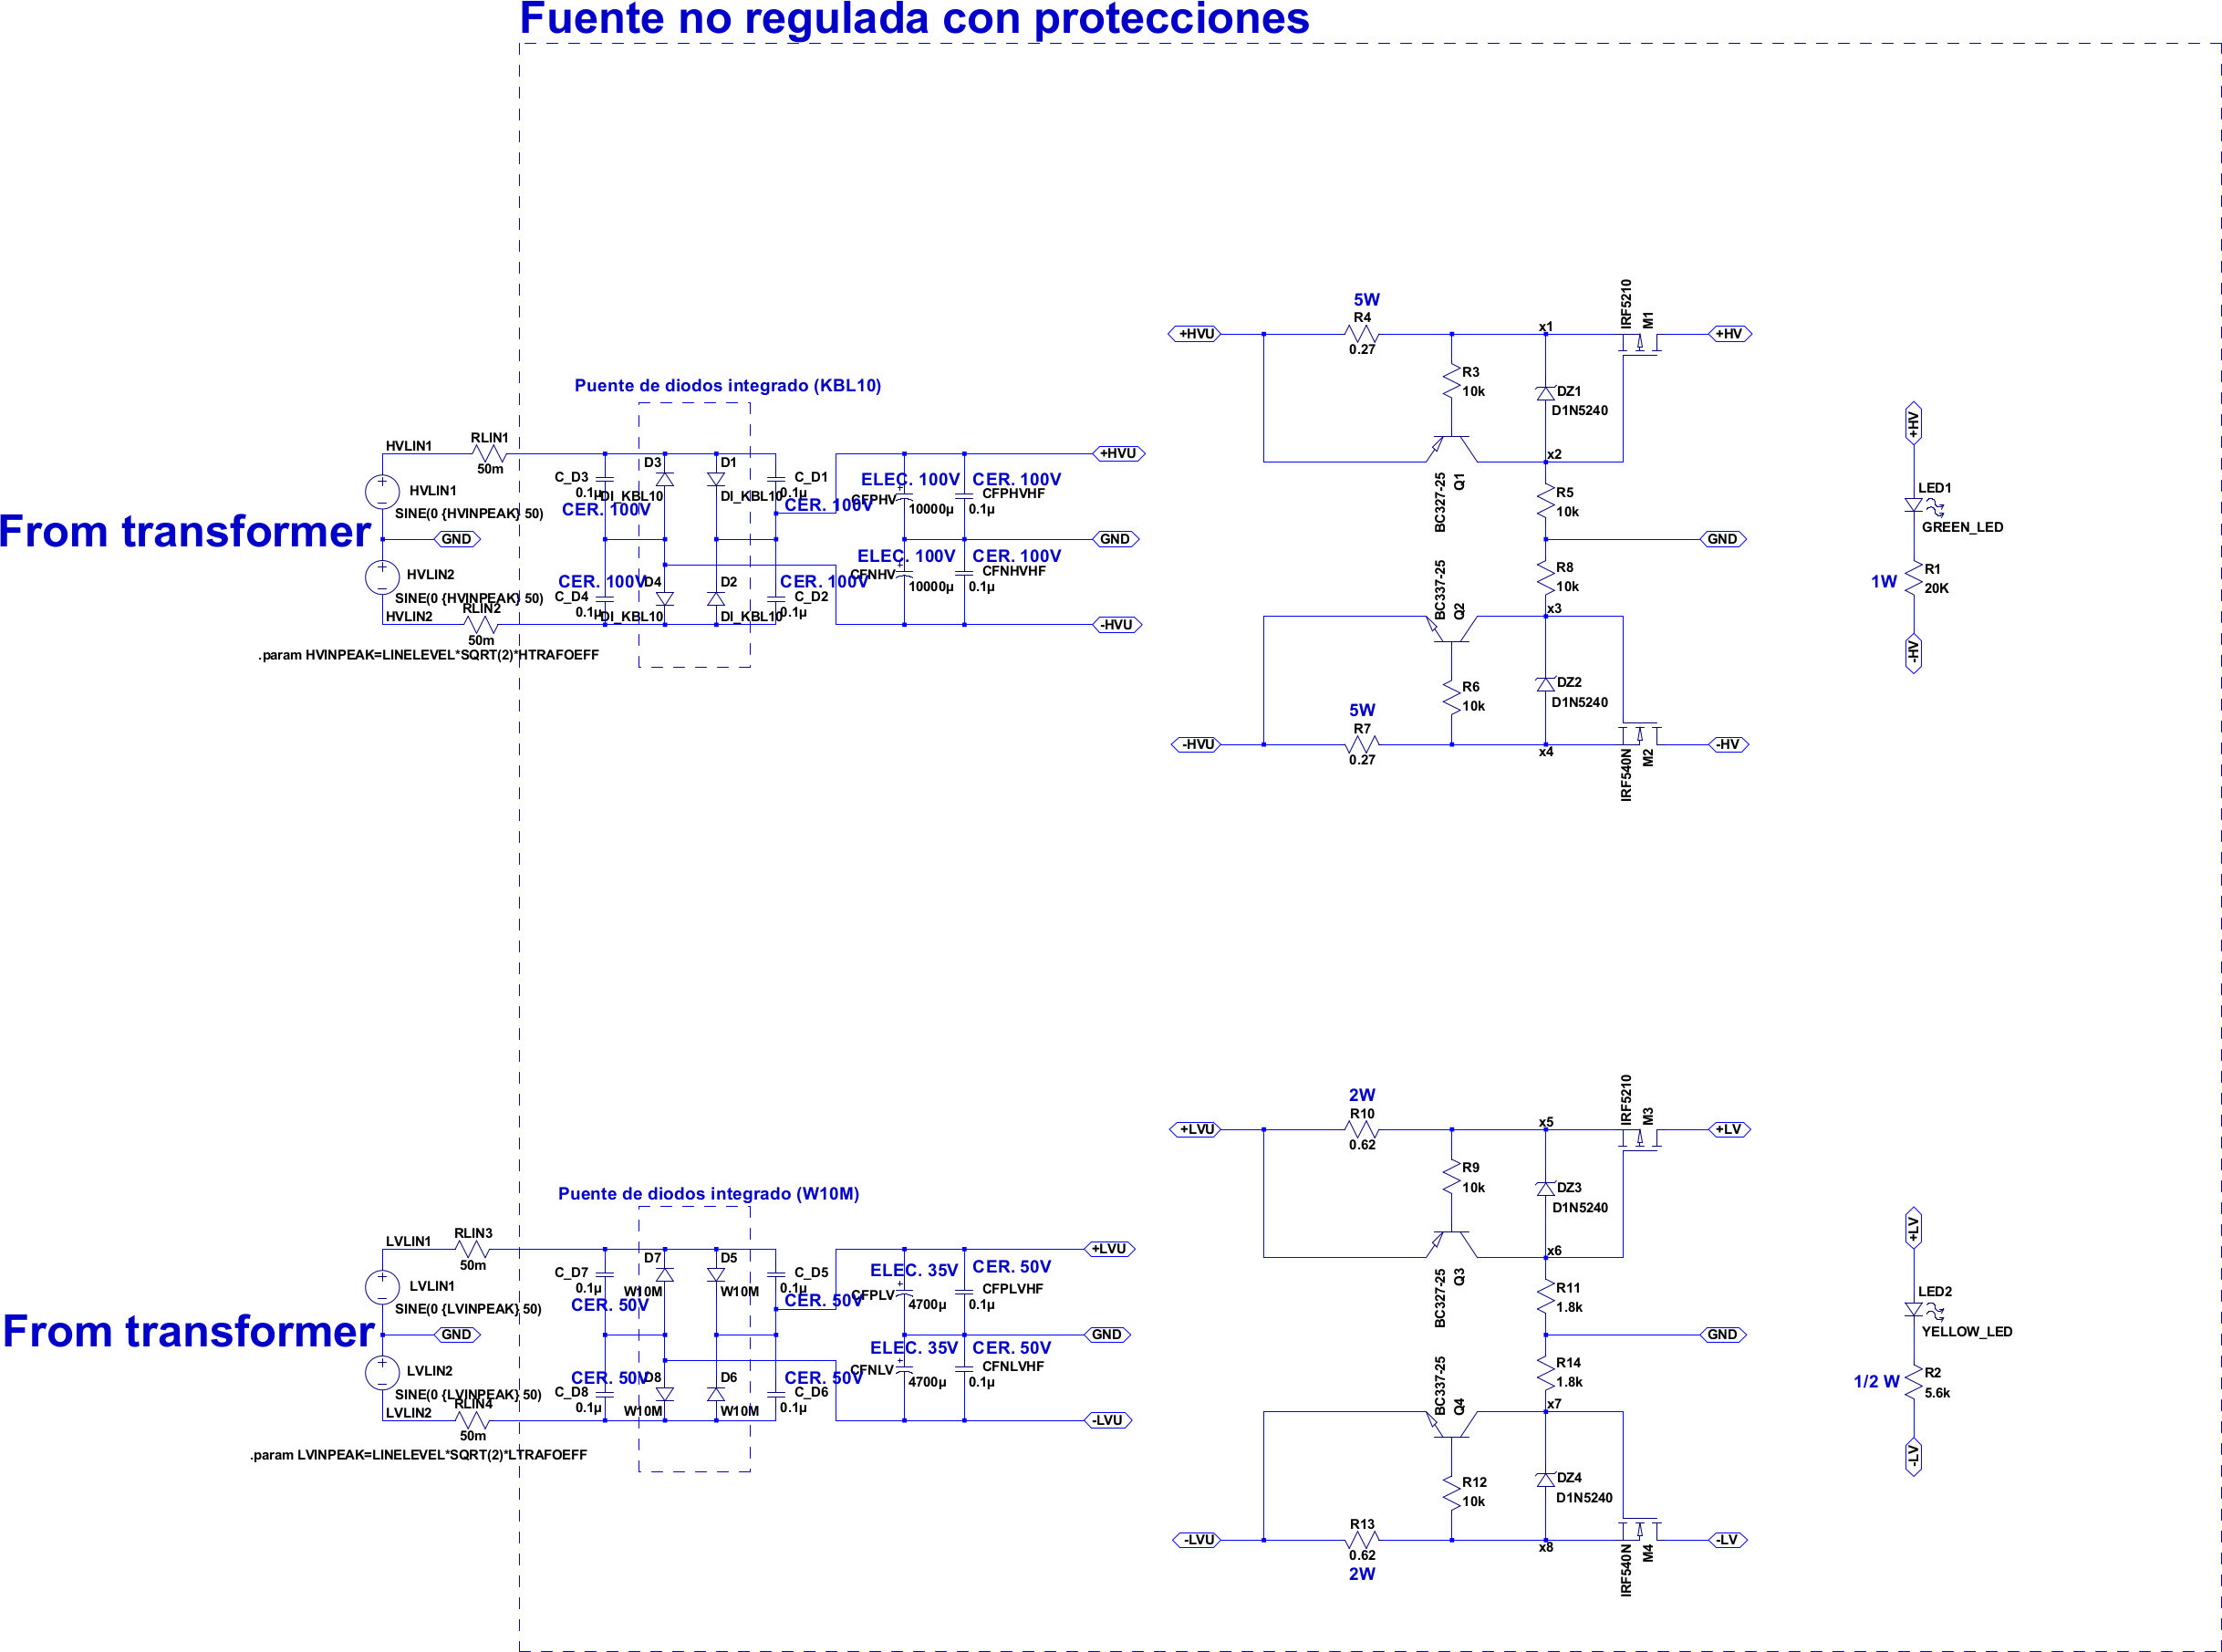
\includegraphics[width=0.7\paperheight, angle=90]{img/power_supply.png}
	\caption{Fuente de alimentación.}
	\label{fig:power_supply}
\end{figure}